\documentclass{article}

\usepackage[utf8]{inputenc}
\usepackage[T1]{fontenc}
\usepackage{geometry}
\usepackage{graphicx}   %ALLOWS INSERTING IMAGES (AND MAYBE SOME MORE STUFF) %
\usepackage{caption}
\usepackage{subcaption} %ALLOWS CAPTIONS FOR SUBFIGURES%
\usepackage{verbatim} % ALLOWS MULTILINE COMMENTS WITH \begin{comment} AND \end{comment} %
\usepackage{amsmath,amssymb} % PERMETTE L'USO DI SIMBOLI MATEMATICI "AVANZATI" COME 'MINORE O UGUALE' E ALTRI %
\usepackage{amstext}
\usepackage{enumitem} %PERMETTE L'USO DI ELENCHI NUMERATI
\usepackage[section]{placeins}

\geometry{a4paper}
                        %Una riga vuota tra due scritte spazia di una riga anche sul pdf. Andare a capo una volta non provoca nulla nel pdf%
\usepackage[italian,english]{babel}
%\usepackage[french, italian]{babel} non funzione per motivi a me ignoti
\frenchspacing 

%%%  INTESTAZIONE  %%%

\title{Relazione dell'esperimento del reticolo olografico}
\author{Alessandro Matteo Rossi}
\date{03 gennaio 2021}



%%%  INIZIO DOCUMENTO  %%%

\begin{document}
\maketitle

%%%  ABSTRACT  %%%
\begingroup
\selectlanguage{english}
\begin{abstract}
    \centering
\end{abstract}
\endgroup


%%%  INDICE  %%%%

\selectlanguage{italian}
\tableofcontents
\newpage

%%%  INTRODUZIONE TEORICA  %%%
%--------------------------------------------------------------------------------------------------------------------------------------------------------------------%
\section{Introduzione teorica}

La luce incidente su un reticolo di diffrazione subisce una diffrazione secondo l'equazione

\begin{equation}
    d(\sin\phi _m(\lambda)+\sin\theta) = m \lambda
    \label{}
\end{equation}

dove $\phi_m$ è l'angolo di diffrazione, funzione della lunghezza d'onda $\lambda$, $\theta$ è l'angolo di incidenza della luce sul reticolo e $m$ è l'ordine. 

\vspace{3mm}

Considerando che la luce utilizzata in ambiente domestico è divergente si hanno molteplici angoli di incidenza $\theta$. Per risolvere questa problematica, non potendo collimare il fascio luminoso con una lente, è conveniente distanziare di una quantità $z$ sufficientemente grande la sorgente luminosa e il reticolo per ottenere una condizione di raggi luminosi incidenti tra loro paralleli (Figura \ref{Schema_Diffrazione}). Ne discende che un sensore ottico posto dietro al reticolo vedrà i raggi come se provenissero dall'infinito, e pertanto con angolo di incidenza $\theta = 0$. Per questa esperienza si è scelto di usare come sensore ottico lo smartphone dello sperimentatore.

\begin{figure}[h]
    \centering
    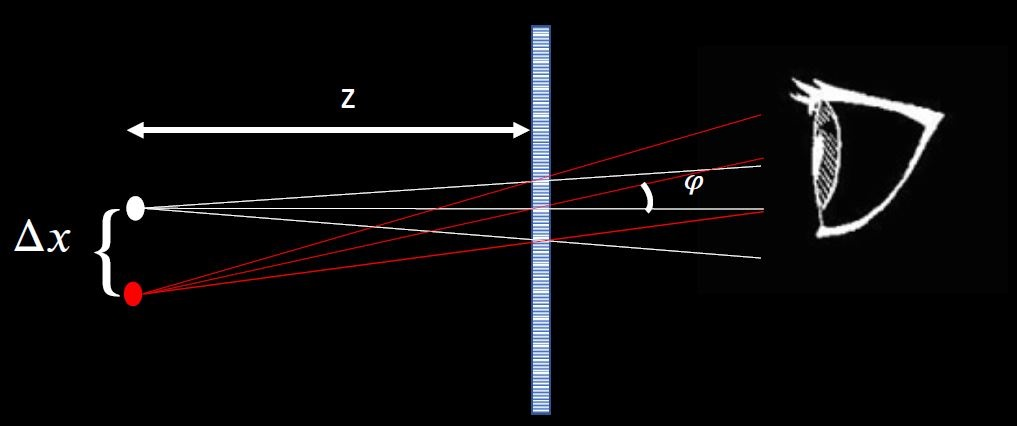
\includegraphics[width=0.55\linewidth]{Schema_Diffrazione.JPG}
    % \caption{}
    \label{Schema_Diffrazione}
\end{figure}
%%%  PROGETTAZIONE DELL'ESPERIENZA  %%%
%--------------------------------------------------------------------------------------------------------------------------------------------------------------------%
\section{Progettazione dell'esperienza}


%%%  PASSO DEL RETICOLO "LUNGO"  %%%
%--------------------------------------------------------------------------------------------------------------------------------------------------------------------%
\section{Passo del reticolo lungo}

%%% LUNGHEZZE D'ONDA EMESSE DA TORCIA A LED %%%
\section{Calcolo lunghezze d'onda emesse da una torcia a led}

%%% CONCLUSIONI %%%
\section{Conclusioni}

%%% APPENDICE %%%
\section{Appendice}



\end{document}